\chapter{Finding symmetries using parameter independence} \label{ch:param-ind}

In \cref{ch:ansatze} the traditional approach of using ansätze to find symmetries of first order ODE:s was used.
There are two main problems with using ansätze.

Firstly, there is a lack of systematics in the process.
There are algorithms that have high success rates at finding symmetries of first order ODE:s that uses a heuristic approach \cite{chebterrab1997computer,chebterrab1998patterns}.
These methods are however not aimed at finding as many symmetries as possible, but rather finding enough symmetries to integrate the system.
If the goal is to draw new biological conclusions from the symmetries, this is insufficient, as the algorithm is considered equally good if it finds the manifest time invariance generated by \(\partial_t\) as if it finds a more biologically interesting symmetry.
Thus such schemes would have to be reevaluated, focusing on metrics such as number of symmetries, and run on collections of ODE:s on forms common in biology.

Secondly, using ansätze to find symmetries gives information about systems unreliably.
Unless the ansatz can be tied to some biological concept independently of the system studied, solving the symmetry conditions using an ansatz only contributes to the knowledge about the systems if new symmetries are found.
Any negative information about which symmetries exist will be hard enough to interpret that it will be discarded in most cases.

In this chapter, a new approach to making the linearized symmetry condition viable to solve for first order ODE:s is presented and used.
The methods central concept is finding symmetries that are independent of one or more parameters of an ODE model.
Its heavily inspired by methods used in group classification introduced by \citeauthor{ovsiannikov1982group} \cite{ovsiannikov1982group}.
The group classification problem centers around models that contain parameters which are not limited to being constants, but instead can be any arbitrary function in the states of the model.
The general biological models described in \cref{ch:models} are special cases of such models, where the parameters are limited to being constants.
This chapter has a description of the method of parameter independence for such models, followed by application of the method to the models under study.

\section{The parameter independence method}

Consider a system of first order ODE:s
\begin{equation} \label[ode]{eq:generic-param-ode}
  \diff{\vb{u}}{t} = \vb*{\omega}(t, \vb{u}; \vb*{\theta})
\end{equation}
with states \(\vb{u} = \left(u^1, \dots, u^s\right)\), parameterized by constant parameters \(\vb*{\theta} = \left(\theta^1, \dots, \theta^m\right)\).
In traditional symmetry calculations, \cref{eq:generic-param-ode} is seen as a single equation, where the parameters \(\vb*{\theta}\) have unknown but fixed values.
Any symmetry found through calculations is a symmetry of the equation defined by that specific set of parameters \(\vb*{\theta}\), which shows itself in symmetry generators themselves containing the parameters.
In contrast, an ODE used in modeling is often seen as a collection of models.
Some parameters might be fixed at the same value in all valid uses of the model, but most parameters are intended to vary over different use cases.
To take biochemistry as an example, while some parameters might indicate the reaction speed between to chemicals (which is seen as fixed), most parameters are intended to vary between conditions the cells are in or between individuals in a cell population.

When interpreting symmetries, the distinction between symmetries for specific instances of the model and symmetries of certain families of the model becomes important.
While there are no known methods to find all the symmetries of a specific system of ODE:s, it is possible to find all symmetries common to a family parameterized by one of the parameters \(\theta^1, \dots, \theta^m\).
Without loss of generality, the one-parameter family of functions
\begin{equation} \label{eq:generic-param-family}
  \Omega = \left\{\diff{\vb{u}}{t} - \vb*{\omega}(t, \vb{u}; \vb*{\theta})\qq*{:} \theta^1 \in S \subseteq \reals \right\}
\end{equation}
with fixed parameters \(\theta^2, \dots, \theta^m\) can be considered.
Call a Lie point symmetry with infinitesimal generator \(X = \xi(x, \vb{u}) \partial_t + \vb*{\eta}(x, \vb{u}) \cdot \partial_{\vb{u}}\) a symmetry of the family of ODE:s defined by
\begin{equation}
  \vb*{\Delta}(\prolong{z}{1}) = 0 \qc \vb*{\Delta} \in \Omega
\end{equation}
if
\begin{equation}
  \eval{\prolong{X}{1}(\vb*{\Delta}(\prolong{z}{1})}_{\vb*{\Delta}(\prolong{z}{1}) = 0} = 0 \qc \forall \vb*{\Delta} \in \Omega.
\end{equation}
Thus, an infinitesimal generator \(X\) of a family of ODE:s defined by \(\Omega\) can not have any dependence on \(\theta^1\).
Evaluating the linearized symmetry condition, the linearized symmetry conditions takes the form
\begin{equation}
  \eta_t - \omega^k \xi_t + \sum_{i=1}^s \omega^i \eta^k_{u^i} - \sum_{i=1}^s \omega^k \omega^i \xi_{u^i} -
  \omega^k_t \xi - \sum_{i=1}^s \omega^k_{u^i} \eta^i = 0 \qc \forall k = 1, \dots, s.
\end{equation}
Since the parameter \(\theta^1\) appears in at least one function \(\omega^j\), and every equation of the linearized symmetry condition includes any \(\omega^j\) at least once, decomposition of the equations in \(\theta^1\) results in a set of at least \(2 s + 1\) equations (taking the \(\omega^k \omega^k\)-term for equation \(k = j\) into account), that will henceforth be called the parameter independence determining equations.
Just like the determining equations for higher order ODE:s, the parameter independence determining equations creates a solvable system of PDE:s, whose solution is the most general form of a symmetry generator for the problem.

This method addresses both previously mentioned weaknesses of using ansätze.
Firstly, the process of finding symmetries by parameter independence is highly systematic.
The method can be used for all parameters of a model, at which point calculations will have revealed all Lie point symmetries independent of one or more of the parameters of the model.
This creates a clear stopping point for calculations.
Secondly, calculations resulting in no parameter independent symmetries being found can still be informative to the modeler since most parameters tend to be connected to some natural concept.

\section{The Gompertz model}
To reiterate, the Gompertz models are\par\noindent
\begin{tabularx}{\linewidth}{rrM}
  Classical, & \(T_i\) :&
  \begin{minipage}{\linewidth}
    \begin{equation}
      \diff{W}{t} = k_G e^{-k_G (t - T_i)} W(t) \label{eq:gompertz-classical-ti^param}
    \end{equation}
  \end{minipage}\tabularnewline
  Classical, & \(W_0\) :&
  \begin{minipage}{\linewidth}
    \begin{equation}
      \diff{W}{t} = k_G \ln(\frac{W_0}{A})e^{-k_G t} W(t) \label{eq:gompertz-classical-w0^param}
    \end{equation}
  \end{minipage}\tabularnewline
  Autonomous, & \(T_i\) and \(W_0\) :&
  \begin{minipage}{\linewidth}
    \begin{equation}
      \diff{W}{t} = -k_G \ln(\frac{W(t)}{A}) W(t) \label{eq:gompertz-autonomous^param}
    \end{equation}
  \end{minipage}\tabularnewline
  System, & \(T_i\) and \(W_0\) :&
  \begin{minipage}{\linewidth}%
    {\begin{subequations}\label{eq:gompertz-system^param}
      \begin{align}
        \diff{W}{t} &= G(t) W(t) \label{eq:gompertz-system-a^param}\\
        \diff{G}{t} &= -k_G G(t). \label{eq:gompertz-system-b^param}
      \end{align}
    \end{subequations}}%
  \end{minipage}
\end{tabularx}

\subsection{The classical Gompertz model}

For the classical Gompertz model, two different parametrizations exist.
For the purposes of the parameter independence method, either of these parametrizations may be used since the parameters \(T_i\) and \(W_0\) only depend on each other and the parameter \(k_G\), but neither the time \(t\) nor the state \(W\).
The \(T_i\) will be used in these calculations.

The linearized symmetry condition \labelcref{eq:linearized-first-order-symmetry} is for the classical \(T_i\)-parameterized Gompertz model
\begin{equation}\label{eq:gompertz-classical-lin-symmetry-cond}
  \begin{split}
    \eta_t &+ k_G e^{-k_G (t - T_i)} W\left(\eta_W - \xi_t\right) - (k_G)^2 e^{-2k_G (t - T_i)} W^2 \xi_W +\\ &+ (k_G)^2 e^{-k_G (t - T_i)} W \xi - k_G e^{-k_G (t - T_i)} \eta = 0.
  \end{split}
\end{equation}
For a generator \(\qty(\xi, \eta)\) to be independent of a parameter, \cref{eq:gompertz-classical-lin-symmetry-cond} is decomposed by functionally independent coefficients of that parameter.

\subsubsection{\texorpdfstring{\(k_G\)-independent symmetries}{Growth rate-independent symmetries}}

Decomposition of \cref{eq:gompertz-classical-lin-symmetry-cond} in \(k_G\) gives the parameter independence determining equations
\begin{subequations}
  \begin{flalign}
    1 & : & \eta_t &= 0 && \FlLabel{eq:gompertz-classical-det-kg-a}\\
    k_G e^{-k_G (t - T_i)} & : & W \left(\eta_W - \xi_t\right) - \eta &= 0 && \FlLabel{eq:gompertz-classical-det-kg-b}\\
    (k_G)^2 e^{-k_G (t - T_i)} & : & W \xi &= 0 && \FlLabel{eq:gompertz-classical-det-kg-c}\\
    (k_G)^2 e^{-2k_G (t - T_i)} & : & W^2 \xi_W &= 0. && \FlLabel{eq:gompertz-classical-det-kg-d}
  \end{flalign}
\end{subequations}
From \cref{eq:gompertz-classical-det-kg-c} it is clear that
\begin{equation}
  \xi \equiv 0,
\end{equation}
and hence \cref{eq:gompertz-classical-det-kg-d} must also hold.
From \cref{eq:gompertz-classical-det-kg-a} it is clear that
\begin{equation}
  \eta = \eta(W)
\end{equation}
is a function only in \(W\).
This leaves \cref{eq:gompertz-classical-det-kg-b} that simplifies into the ODE
\begin{equation}
  W \eta_W - \eta = 0
\end{equation}
with the general solution
\begin{equation}
  \eta = c_1 W,
\end{equation}
where \(c_1\) is an arbitrary constant.
Thus any \(k_G\)-independent symmetry generator of the classical Gompertz model \labelcref{eq:gompertz-classical-ti^param} must have the form
\begin{align}
  \xi &= 0 \\
  \eta &= c_1 W,
\end{align}
which is spanned by the generator basis
\begin{equation}
  X_{\text{c},4} = W \partial_W.
\end{equation}

\subsubsection{\texorpdfstring{\(T_i\)-independent symmetries}{Inflection time-independent symmetries}}

Decomposition of \cref{eq:gompertz-classical-lin-symmetry-cond} in \(T_i\) gives the parameter independence determining equations
\begin{subequations}
  \begin{flalign}
    1 & : & \eta_t &= 0 && \FlLabel{eq:gompertz-classical-det-ti-a}\\
    e^{k_G T_i} & : & k_G e^{-k_G t} W \left(\eta_W - \xi_t\right) + (k_G)^2 e^{-k_G t} W \xi - k_G e^{-k_G t} \eta &= 0 && \FlLabel{eq:gompertz-classical-det-ti-b}\\
    e^{2 k_G T_i} & : & -(k_G)^2 e^{-2 k_G t} W^2 \xi_W &= 0 && \FlLabel{eq:gompertz-classical-det-ti-c}
  \end{flalign}
\end{subequations}
From \cref{eq:gompertz-classical-det-ti-a,eq:gompertz-classical-det-ti-c} it is clear that
\begin{align}
  \eta &= \eta(W) \\
  \xi &= \xi(t)
\end{align}
respectively.
Dividing \cref{eq:gompertz-classical-det-ti-b} by \(k_G e^{-k_G t}\) shows that
\begin{equation}\label{eq:gompertz-classical-det-ti-b-simple}
  W \left(\eta_W - \xi_t\right) + k_G W \xi - \eta = 0.
\end{equation}
Since \(\xi\) (and thus its derivative) is the only source of time dependence in \cref{eq:gompertz-classical-det-ti-b-simple},
\begin{equation}
  k_G W \xi - W \xi_t = f(W).
\end{equation}
for some function \(f\) in \(W\).
And since \(\xi\) (and thus its derivative) are functions only in \(t\)
\begin{equation}
  k_G \xi - \xi_t = c_1,
\end{equation}
where \(c_1\) is an arbitrary constant, which in turn has the general solution
\begin{equation}
  \xi = c_2 e^{k_G t} + \frac{c_1}{k_G}
\end{equation}
with an additional arbitrary constant \(c_2\).
Insertion of this result in \cref{eq:gompertz-classical-det-ti-b-simple} yields
\begin{equation}
  W \eta_W - \eta + c_1 W = 0,
\end{equation}
which, since \(\eta\) is only a function in \(W\), is a straight forward ODE with the general solution
\begin{equation}
  \eta = -c_1 W \ln(W) + c_3 W.
\end{equation}
Thus any \(T_i\)-independent symmetry generator of the classical Gompertz model \labelcref{eq:gompertz-classical-ti^param} must have the form
\begin{align}
  \xi &= \frac{c_1}{k_G} + c_2 e^{k_G t} \\
  \eta &= -c_1 W \ln(W) + c_3 W,
\end{align}
which is spanned by the generator basis
\begin{align}
  X_{\text{c},1} &= e^{k_G t} \partial_t \\
  X_{\text{c},4} &= W \partial_W \\
  X_{\text{c},5} &= \partial_t - k_G W \ln(W) \partial_W.
\end{align}

\subsubsection{All of the found generators}
The basis of all the generators found by the parameter independence method for the classical Gompertz model are
\begin{align}
  X_{\text{c},1} &= e^{k_G t} \partial_t \\
  X_{\text{c},4} &= W \partial_W \\
  X_{\text{c},5} &= \partial_t - k_G W \ln(W) \partial_W.
\end{align}
The corresponding transformations can be seen in \cref{fig:gompertz-classical-param}.
\begin{figure}
  \centering
  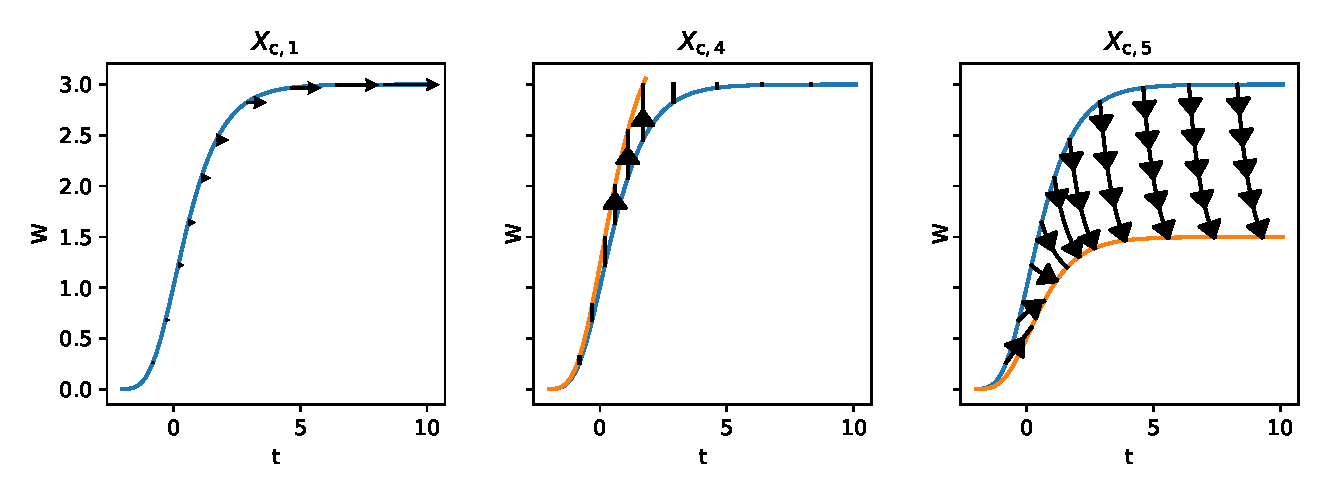
\includegraphics[width=.96\textwidth]{images/gompertz-classical-param}
  \caption{Representative transformations of the Lie groups corresponding to symmetry generators of the classical Gompertz model found using the parameter independence method.}
  \label{fig:gompertz-classical-param}
\end{figure}


\subsection{The autonomous Gompertz model}

For the autonomous Gompertz model there is only one parametrization of interest.
The linearized symmetry condition \labelcref{eq:linearized-first-order-symmetry} is for the autonomous Gompertz model
\begin{equation}\label{eq:gompertz-autonomous-lin-symmetry-cond}
  \begin{split}
    \eta_t &- k_G \ln(\frac{W}{A}) W\left(\eta_W - \xi_t\right) - (k_G)^2 \left(\ln(\frac{W(t)}{A})\right)^2 W^2 \xi_W +\\ &+ k_G \left(\ln(\frac{W}{A}) + 1\right) \eta = 0.
  \end{split}
\end{equation}

\subsubsection{\texorpdfstring{\(k_G\)-independent symmetries}{Growth rate-independent symmetries}}

Decomposition of \cref{eq:gompertz-autonomous-lin-symmetry-cond} in \(k_G\) gives the parameter independence determining equations
\begin{subequations}
  \begin{flalign}
    1 & : & \eta_t &= 0 && \FlLabel{eq:gompertz-autonomous-det-kg-a}\\
    k_G & : & -\ln(\frac{W}{A}) W\left(\eta_W - \xi_t\right) + \left(\ln(\frac{W}{A}) + 1\right) \eta &= 0 && \FlLabel{eq:gompertz-autonomous-det-kg-b}\\
    (k_G)^2 & : & -\left(\ln(\frac{W(t)}{A})\right)^2 W^2 \xi_W &= 0. && \FlLabel{eq:gompertz-autonomous-det-kg-c}
  \end{flalign}
\end{subequations}
From \cref{eq:gompertz-autonomous-det-kg-a,eq:gompertz-autonomous-det-kg-c}
\begin{align}
  \eta &= \eta(W) \\
  \xi = \xi(t).
\end{align}
Hence, since the only source of time dependence in \cref{eq:gompertz-autonomous-det-kg-b} is \(\xi_t\),
\begin{equation}
  \xi_t = c_1
\end{equation}
where \(c_1\) is an arbitrary constant, and thus
\begin{equation}
  \xi = c_2 t + c_1
\end{equation}
for an additional arbitrary constant \(c_2\).
\Cref{eq:gompertz-autonomous-det-kg-b} can thus be rewritten as
\begin{equation}
  \eta_W - \frac{\ln(\frac{W}{A}) + 1}{\ln(\frac{W}{A}) W} \eta - c_1 = 0,
\end{equation}
which is a scalar first order ODE with the solution
\begin{equation}
  \eta = c_1 \ln(\ln(\frac{W}{A})) \ln(\frac{W}{A}) W + c_3 \ln(\frac{W}{A}) W.
\end{equation}
Thus any \(k_G\)-independent symmetry generator of the autonomous Gompertz model \labelcref{eq:gompertz-autonomous^param} must have the form
\begin{align}
  \xi &= c_2 + c_1 t \\
  \eta &= c_1 \ln(\ln(\frac{W}{A})) \ln(\frac{W}{A}) W + c_3 \ln(\frac{W}{A}) W,
\end{align}
which is spanned by the generator basis
\begin{align}
  X_{\text{a},3} &= \ln(\frac{W}{A}) W \partial_W \\
  X_{\text{a},4} &= \partial_t \\
  X_{\text{a},5} &= t \partial_t + \ln(\ln(\frac{W}{A})) \ln(\frac{W}{A}) W \partial_W.
\end{align}

\subsubsection{\texorpdfstring{\(A\)-independent symmetries}{Carrying capacity-independent symmetries}}

Decomposition of \cref{eq:gompertz-autonomous-lin-symmetry-cond} in \(A\) gives the parameter independence determining equations
\begin{subequations}
  \begin{flalign}
    1 & : & \eta_t + k_G \eta &= 0 && \FlLabel{eq:gompertz-autonomous-det-a-a}\\
    \ln(\frac{W}{A}) & : & - k_G W\left(\eta_W - \xi_t\right)  + k_G \eta &= 0 && \FlLabel{eq:gompertz-autonomous-det-a-b}\\
    \left(\ln(\frac{W}{A})\right)^2 & : & - (k_G)^2 W^2 \xi_W &= 0. && \FlLabel{eq:gompertz-autonomous-det-a-c}
  \end{flalign}
\end{subequations}
From \cref{eq:gompertz-autonomous-det-a-c}
\begin{equation}
  \xi = \xi(t).
\end{equation}
Since \(\eta\) (and thus its derivative) are the only unknown sources of \(W\)-dependence in \cref{eq:gompertz-autonomous-det-a-b},
\begin{equation}
  \eta_W - \frac{1}{W}\eta = \xi_t(t)
\end{equation}
must hold.
Integration in \(W\) gives
\begin{equation}
  \eta = \ln(W) W \xi_t(t) + W f(t)
\end{equation}
for some arbitrary function \(f\) in time.
Inserting this result in \cref{eq:gompertz-autonomous-det-a-a} gives
\begin{equation}
  \ln(W) W \xi_{tt} + W f_t + k_G \ln(W) W \xi_t + k_G W f
\end{equation}
which can be decomposed by \(W\) into
\begin{align}
  \xi_{tt} + k_G \xi_t &= 0 \\
  f_t + k_G f &= 0
\end{align}
with solutions
\begin{align}
  \xi &= - c_1 \frac{1}{k_G} e^{-k_G t} + c_2 \\
  f &= c_3 e^{-k_G t}.
\end{align}
Thus any \(A\)-independent symmetry generator of the autonomous Gompertz model \labelcref{eq:gompertz-autonomous^param} must have the form
\begin{align}
  \xi &= - c_1 \frac{1}{k_G} e^{-k_G t} + c_2 \\
  \eta &= c_1 e^{-k_G t} \ln(W) W  + c_3 e^{-k_G t} W,
\end{align}
which is spanned by the generator basis
\begin{align}
  X_{\text{a},2} &= e^{-k_G t} W \partial_W \\
  X_{\text{a},4} &= \partial_t \\
  X_{\text{a},6} &= e^{-k_G t} \partial_t - k_G e^{-k_G t} \ln(W) W \partial_W.
\end{align}

\subsubsection{All found generators}
The basis of all the generators found by the parameter independence method for the autonomous Gompertz model are
\begin{align}
  X_{\text{a},2} &= e^{-k_G t} W \partial_W \\
  X_{\text{a},3} &= \ln(\frac{W}{A}) W \partial_W \\
  X_{\text{a},4} &= \partial_t \\
  X_{\text{a},5} &= t \partial_t + \ln(\abs{\ln(\frac{W}{A})}) \ln(\frac{W}{A}) W \partial_W \\
  X_{\text{a},6} &= e^{-k_G t} \partial_t - k_G e^{-k_G t} \ln(W) W \partial_W.
\end{align}
The corresponding transformations can be seen in \cref{fig:gompertz-autonomous-param}.
\begin{figure}
  \centering
  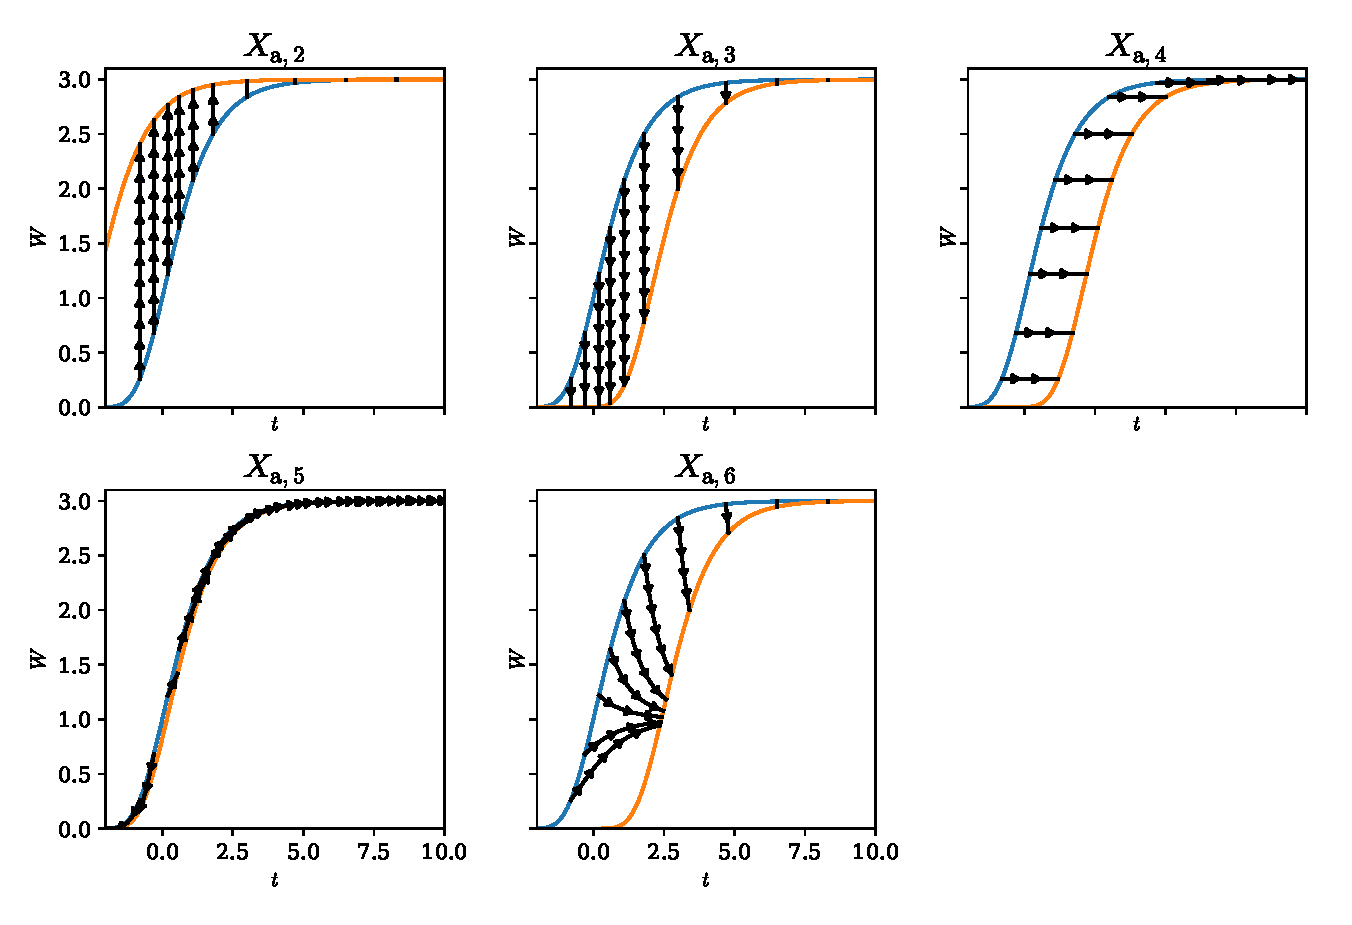
\includegraphics[width=.96\textwidth]{images/gompertz-autonomous-param}
  \caption{Representative transformations of the Lie groups corresponding to symmetry generators of the autonomous Gompertz model found using the parameter independence method.}
  \label{fig:gompertz-autonomous-param}
\end{figure}

\subsection{The system Gompertz model}

For the system Gompertz model there is also only one parametrization of interest.
The linearized symmetry condition \labelcref{eq:linearized-first-order-symmetry} is for the system Gompertz model
\begin{subequations}\label{eq:gompertz-system-lin-symmetry-cond}
  \begin{align}
    \begin{split}\label{eq:gompertz-system-lin-symmetry-cond-a}
      \eta^1_t + W G \left(\eta^1_W - \xi_t\right) -k_G G \eta^1_G - W^2 G^2 \xi_W +&\\+ k_G W G^2 \xi_G - G \eta^1 - W \eta^2 &= 0 
    \end{split}\\
    \begin{split}\label{eq:gompertz-system-lin-symmetry-cond-b}
      \eta^2_t - k_G G \left(\eta^2_G - \xi_t\right) + W G \eta^2_G + k_G W G^2 \xi_W -&\\- (k_G)^2 G^2 \xi_G + k_G \eta^2 &= 0. 
    \end{split}
  \end{align}
\end{subequations}

\subsubsection{\texorpdfstring{\(k_G\)-independent symmetries}{Growth rate-independent symmetries}}

Decomposition of \cref{eq:gompertz-system-lin-symmetry-cond} in \(k_G\) gives the parameter independence determining equations
\begin{subequations}
  \begin{flalign}
    \labelcref{eq:gompertz-system-lin-symmetry-cond-a},\ & 1 : & \eta^1_t + W G \left(\eta^1_W - \xi_t\right) - W^2 G^2 \xi_W - G \eta^1 - W \eta^2 &= 0 && \FlLabel{eq:gompertz-system-det-kg-a}\\
    \labelcref{eq:gompertz-system-lin-symmetry-cond-a},\ & k_G : & - G \eta^1_G + W G^2 \xi_G &= 0 && \FlLabel{eq:gompertz-system-det-kg-b}\\
    \labelcref{eq:gompertz-system-lin-symmetry-cond-b},\ & 1 : & \eta^2_t + W G \eta^2_G &= 0. && \FlLabel{eq:gompertz-system-det-kg-c} \\
    \labelcref{eq:gompertz-system-lin-symmetry-cond-b},\ & k_G : & - G \left(\eta^2_G - \xi_t\right) + W G^2 \xi_W + \eta^2 &= 0. && \FlLabel{eq:gompertz-system-det-kg-d} \\
    \labelcref{eq:gompertz-system-lin-symmetry-cond-b},\ & (k_G)^2 : & - G^2 \xi_G &= 0. && \FlLabel{eq:gompertz-system-det-kg-e}
  \end{flalign}
\end{subequations}
From \cref{eq:gompertz-system-det-kg-e} it is clear that
\begin{equation}
  \xi = \xi(t, W),
\end{equation}
and thus from \cref{eq:gompertz-system-det-kg-b}
\begin{equation}
  \eta^1 = \eta^1(t, W).
\end{equation}
From \cref{eq:gompertz-system-det-kg-a}
\begin{equation}
  \eta^2 = \frac{1}{W}\eta^1_t + G \left(\eta^1_W - \xi_t - \frac{1}{W} \eta^1 \right) - W G^2 \xi_W,
\end{equation}
and thus \cref{eq:gompertz-system-det-kg-d} can be written as
\begin{equation}\label{eq:gompertz-system-det-kg-d-simple}
  \frac{1}{W}\eta^1_t + G \xi_t + 2 G^2 W \xi_W = 0.
\end{equation}
Since both \(\xi\) and \(\eta^1\) are not functions in \(G\), \cref{eq:gompertz-system-det-kg-d-simple} can be decomposed in \(G\) giving
\begin{align}
  \xi_t &= 0\\
  \xi_W &= 0\\
  \eta^1_t &= 0.
\end{align}
Thus
\begin{align}
  \xi &= c_1\\
  \eta^1 &= \eta^1(W)
  \eta^2 &= G \left(\eta^1_W(W) - \frac{1}{W} \eta^1(W) \right),
\end{align}
where \(c_1\) is an arbitrary constant, and \cref{eq:gompertz-system-det-kg-c} reduces to
\begin{equation}
  W G^2 \left(\eta^1_W - \frac{1}{W} \eta^1 \right)_W = 0.
\end{equation}
Thus the ODE
\begin{equation}
  \eta^1_W - \frac{1}{W} \eta^1 = c_2
\end{equation}
must hold for an arbitrary constant \(c_2\), which has the general solution
\begin{equation}
  \eta^1 = c_2 \ln(W) W + c_3 W.
\end{equation}
Thus any \(k_G\)-independent symmetry generator of the system Gompertz model \labelcref{eq:gompertz-system^param}\ghostref{eq:gompertz-system-a^param}\ghostref{eq:gompertz-system-b^param} must have the form
\begin{align}
  \xi &= c_1 \\
  \eta^1 &= c_2 \ln(W) W + c_3 W\\
  \eta^2 &= c_2 G
\end{align}
which is spanned by the generator basis
\begin{align}
  X_{\text{s},1} &= \partial_t \\
  X_{\text{s},4} &= W \partial_W \\
  X_{\text{s},6} &= \ln(W) W \partial_W + G \partial_G.
\end{align}
The corresponding transformations can be seen in \cref{fig:gompertz-system-param}.
\begin{figure}
  \centering
  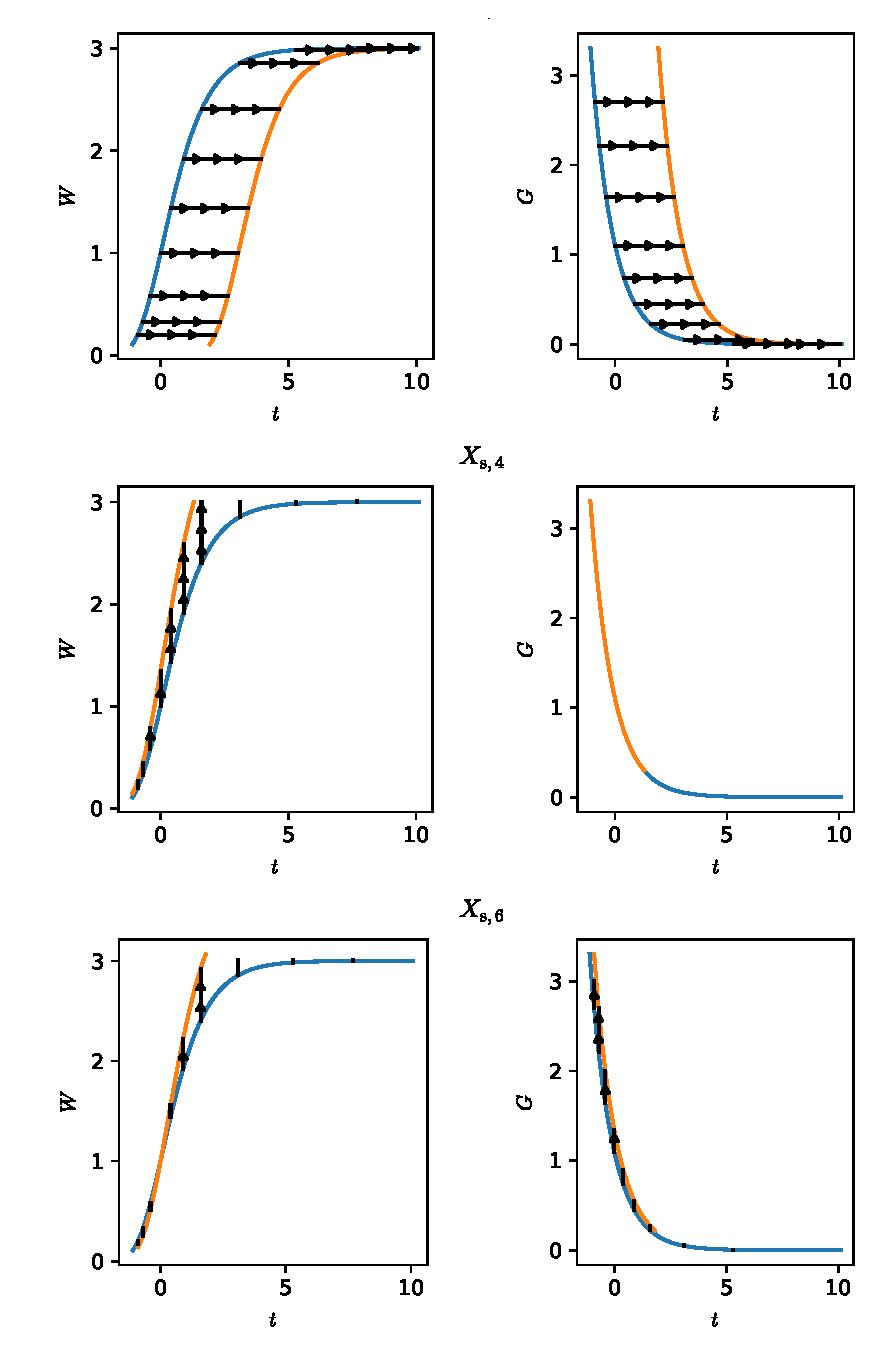
\includegraphics[height=.48\textheight]{images/gompertz-system-param}
  \caption{Representative transformations of the Lie groups corresponding to symmetry generators of the system Gompertz model found using the parameter independence method.}
  \label{fig:gompertz-system-param}
\end{figure}

\section{The Lotka--Volterra model}

The linearized symmetry condition \labelcref{eq:linearized-general-symmetry} is for the Lotka--Volterra model
\begin{subequations}\label{eq:lotka-volterra-lin-symmetry-cond}
  \begin{align}
    \begin{split}
      \eta^1_t &+ \qty(a N - b N) \qty(\eta^1_{N} - \xi_t) + \qty(c N P - d P) \eta^1_{P} - \qty(a N - b N P)^2 \xi_{N} -\\
      &- \qty(a N - b N P) \qty(c N P - d P) \xi_{P} - \qty(a - b P) \eta^1 + b N \eta^2 = 0
    \end{split}\\
    \begin{split}
      \eta^2_t &+ \qty(a N - b N P) \eta^2_{N} + \qty(c N P - d P) \qty(\eta^2_{P} - \xi_t) -\\
      &- \qty(a N - b N P) \qty(c N P - d P) \xi_{N} - \qty(c N P - d P)^2 \xi_{P} - c P \eta^1 -\\
      &- \qty(c N - d) \eta^2 = 0.
    \end{split}
  \end{align}
\end{subequations}

\subsubsection{\texorpdfstring{\(a\)-independent symmetries}{a-independent symmetries}}

Decomposition of \cref{eq:lotka-volterra-lin-symmetry-cond} in \(a\) gives the parameter independence determining equations
\begin{subequations}\label{eq:lotka-volterra-det-a}
  \begin{flalign}
    \diff{N}{t}, 1 & : & - N^{2} P^{2} b^{2} \xi_{N} - N P b \eta^1_{N} + N P b \xi_{t} + N b \eta^{2} + P b \eta^{1} +&&&\\
    &&\quad+ \left(N P c - P d\right) \eta^1_{P} + \left(N^{2} P^{2} b c - N P^{2} b d\right) \xi_{P} + \eta^1_{t} &= 0 && \FlLabel{eq:lotka-volterra-det-a-a}\\
    \diff{N}{t}, a & : & 2 N^{2} P b \xi_{N} + N \eta^1_{N} - N \xi_{t} + \left(- N^{2} P c + N P d\right) \xi_{P} -&&&\\
    &&\quad- \eta^{1} &= 0 && \FlLabel{eq:lotka-volterra-det-a-b}\\
    \diff{N}{t}, a^2 & : & - N^{2} \xi_{N} &= 0 && \FlLabel{eq:lotka-volterra-det-a-c}\\
    \diff{P}{t}, 1 & : & - N P b \eta^2_{N} - P c \eta^{1} + \left(- N c + d\right) \eta^{2} +&&&\\
    &&\quad+  \left(- N P c + P d\right) \xi_{t} + \left(N P c - P d\right) \eta^2_{P} +&&&\\
    &&\quad+ \left(N^{2} P^{2} b c - N P^{2} b d\right) \xi_{N} +&&&\\
    &&\quad+ \left(- N^{2} P^{2} c^{2} + 2 N P^{2} c d - P^{2} d^{2}\right) \xi_{P} + \eta^2_{t} &= 0 && \FlLabel{eq:lotka-volterra-det-a-d}\\
    \diff{P}{t}, a & : & N \eta^2_{N} + \left(- N^{2} P c + N P d\right) \xi_{N} &= 0. && \FlLabel{eq:lotka-volterra-det-a-e}
  \end{flalign}
\end{subequations}
From \cref{eq:lotka-volterra-det-a-c,eq:lotka-volterra-det-a-e} it is clear that
\begin{align}
  \eta^2 &= \eta^2(t, P)\\
  \xi &= \xi(t, P),
\end{align}
and thus \cref{eq:lotka-volterra-det-a-d} can be written as
\begin{align}
  \begin{split}
    \eta^{1} =& \left(- N + \frac{d}{c}\right) \xi_{t} + \left(N - \frac{d}{c}\right) \eta^2_{P} + \left(- \frac{N}{P} + \frac{d}{P c}\right) \eta^{2} +\\
    &+ \left(- N^{2} P c + 2 N P d - \frac{P d^{2}}{c}\right) \xi_{P} + \frac{\eta^2_{t}}{P c}.
  \end{split}
\end{align}
Since neither \(\xi\) nor \(\eta^2\) depends on \(N\), and \(\eta^1\) thus only depends explicitly on \(N\), the remaining parameter independence determining equations \labelcref{eq:lotka-volterra-det-a-a,eq:lotka-volterra-det-a-b} can be decomposed further in \(N\) resulting in the equations
\begin{subequations}
  \begin{align}
    - 2 P c \xi_{P} &= 0 \label{eq:lotka-volterra-det-aN-a}\\
    P d \xi_{P} - \xi_{t} &= 0 \label{eq:lotka-volterra-det-aN-b}\\
    \frac{P d^{2} \xi_{P}}{c} + \frac{d \eta^2_{P}}{c} - \frac{d \xi_{t}}{c} - \frac{d \eta^{2}}{P c} - \frac{\eta^2_{t}}{P c} &= 0 \label{eq:lotka-volterra-det-aN-c}\\
    - P^{2} c^{2} \xi_{PP} - P c^{2} \xi_{P} &= 0 \label{eq:lotka-volterra-det-aN-d}\\
    3 P^{2} c d \xi_{PP} + P c \eta^2_{PP} - 2 P c \xi_{Pt} - c \eta^2_{P} + \left(2 P^{2} b c + 3 P c d\right) \xi_{P} + \frac{c \eta^{2}}{P} &= 0 \label{eq:lotka-volterra-det-aN-e}\\
    \begin{split}\label{eq:lotka-volterra-det-aN-f}
      - 3 P^{2} d^{2} \xi_{PP} + P b \xi_{t} - 2 P d \eta^2_{PP} + 4 P d \xi_{Pt} + 2 d \eta^2_{P} + \left(b - \frac{2 d}{P}\right) \eta^{2} +&\\
      + \left(- P^{2} b d - 3 P d^{2}\right) \xi_{P} - \xi_{tt} + 2 \eta^2_{Pt} - \frac{2 \eta^2_{t}}{P} &= 0
    \end{split}\\
    \begin{split}\label{eq:lotka-volterra-det-aN-g}
      \frac{P^{2} d^{3} \xi_{PP}}{c} + \frac{P b d \xi_{t}}{c} + \frac{P d^{2} \eta^2_{PP}}{c} - \frac{2 P d^{2} \xi_{Pt}}{c} + \left(\frac{b}{c} + \frac{2 d}{P c}\right) \eta^2_{t} +&\\
      + \left(\frac{b d}{c} + \frac{d^{2}}{P c}\right) \eta^{2} + \left(- \frac{P b d}{c} - \frac{d^{2}}{c}\right) \eta^2_{P} + \left(- \frac{P^{2} b d^{2}}{c} + \frac{P d^{3}}{c}\right) \xi_{P} +&\\
      + \frac{d \xi_{tt}}{c} - \frac{2 d \eta^2_{Pt}}{c} + \frac{\eta^2_{tt}}{P c} &= 0.
    \end{split}
  \end{align}
\end{subequations}
\Cref{eq:lotka-volterra-det-aN-a,eq:lotka-volterra-det-aN-b} gives that
\begin{equation}
  \xi = c_1,
\end{equation}
where \(c_1\) is an arbitrary constant.
Thus the remaining \cref{eq:lotka-volterra-det-aN-c,eq:lotka-volterra-det-aN-e,eq:lotka-volterra-det-aN-f,eq:lotka-volterra-det-aN-g} simplify to
\begin{subequations}
  \begin{align}
    \frac{d \eta^2_{P}}{c} - \frac{d \eta^{2}}{P c} - \frac{\eta^2_{t}}{P c} &= 0 \label{eq:lotka-volterra-det-aN-c-simp}\\
    P c \eta^2_{PP} - c \eta^2_{P} + \frac{c \eta^{2}}{P} &= 0 \label{eq:lotka-volterra-det-aN-e-simp}\\
    - 2 P d \eta^2_{PP} + 2 d \eta^2_{P} + \left(b - \frac{2 d}{P}\right) \eta^{2} + 2 \eta^2_{Pt} - \frac{2 \eta^2_{t}}{P} &= 0 \label{eq:lotka-volterra-det-aN-f-simp}\\
    \begin{split}
      \frac{P d^{2} \eta^2_{PP}}{c} + \left(\frac{b}{c} + \frac{2 d}{P c}\right) \eta^2_{t} + \left(\frac{b d}{c} + \frac{d^{2}}{P c}\right) \eta^{2} +&\\
      + \left(- \frac{P b d}{c} - \frac{d^{2}}{c}\right) \eta^2_{P} - \frac{2 d \eta^2_{Pt}}{c} + \frac{\eta^2_{tt}}{P c} &= 0.
    \end{split}
  \end{align}
\end{subequations}
\Cref{eq:lotka-volterra-det-aN-c-simp} has the general solution
\begin{equation}
  \eta^{2} = F{\left(P e^{d t} \right)} e^{- d t}
\end{equation}
for an arbitrary univariate function \(F\).
Thus \cref{eq:lotka-volterra-det-aN-e-simp,eq:lotka-volterra-det-aN-f-simp} can be further simplified to
\begin{align}
  P c e^{d t} F''{\left(P e^{d t} \right)} - c F'{\left(P e^{d t} \right)} + \frac{c F{\left(P e^{d t} \right)} e^{- d t}}{P} &= 0 \label{eq:lotka-volterra-det-aN-e-simp2}\\
  b F{\left(P e^{d t} \right)} e^{- d t} &= 0. \label{eq:lotka-volterra-det-aN-f-simp2}
\end{align}
Thus it clear from \cref{eq:lotka-volterra-det-aN-f-simp2} that
\begin{equation}
  F \equiv 0
\end{equation}
and hence the general solution to the parameter independence determining equations \labelcref{eq:lotka-volterra-det-a} is
\begin{align}
  \xi &= c_1 \\
  \eta^1 &= 0\\
  \eta^2 &= 0
\end{align}
which is spanned by the manifest generator
\begin{equation}
  X_1 = \partial_t.
\end{equation}

\subsubsection{\texorpdfstring{\(b\)-independent symmetries}{b-independent symmetries}}

Decomposition of \cref{eq:lotka-volterra-lin-symmetry-cond} in \(b\) gives the parameter independence determining equations
\begin{subequations}\label{eq:lotka-volterra-det-b}
  \begin{flalign}
    \diff{N}{t}, 1 & : & - N^{2} a^{2} \xi_{N} + N a \eta^1_{N} - N a \xi_{t} - a \eta^{1} + \left(N P c - P d\right) \eta^1_{P} +&&&\\&&+ \left(- N^{2} P a c + N P a d\right) \xi_{P} + \eta^1_{t} &= 0 && \FlLabel{eq:lotka-volterra-det-b-a}\\
    \diff{N}{t}, b & : & 2 N^{2} P a \xi_{N} - N P \eta^1_{N} + N P \xi_{t} + N \eta^{2} + P \eta^{1} +&&&\\&&+ \left(N^{2} P^{2} c - N P^{2} d\right) \xi_{P} &= 0 && \FlLabel{eq:lotka-volterra-det-b-b}\\
    \diff{N}{t}, b^2 & : & - N^{2} P^{2} \xi_{N} &= 0 && \FlLabel{eq:lotka-volterra-det-b-c}\\
    \diff{P}{t}, 1 & : & N a \eta^2_{N} - P c \eta^{1} + \left(- N c + d\right) \eta^{2} + \left(- N P c + P d\right) \xi_{t} +&&&\\&&+ \left(N P c - P d\right) \eta^2_{P} + \left(- N^{2} P a c + N P a d\right) \xi_{N} +&&&\\&&+ \left(- N^{2} P^{2} c^{2} + 2 N P^{2} c d - P^{2} d^{2}\right) \xi_{P} + \eta^2_{t} &= 0 && \FlLabel{eq:lotka-volterra-det-b-d}\\
    \diff{P}{t}, b & : & - N P \eta^2_{N} + \left(N^{2} P^{2} c - N P^{2} d\right) \xi_{N} &= 0. && \FlLabel{eq:lotka-volterra-det-b-e}
  \end{flalign}
\end{subequations}
From \cref{eq:lotka-volterra-det-b-c,eq:lotka-volterra-det-b-e} it is clear that
\begin{align}
  \xi &= \xi(t, P) \\
  \eta^2 &= \eta^2(t, P),
\end{align}
and thus \cref{eq:lotka-volterra-det-b-d} can be written as
\begin{multline}
  \eta^{1} = - N^{2} P c \xi_{P} + 2 N P d \xi_{P} + N \eta^2_{P} - N \xi_{t} -\\- \frac{N \eta^{2}}{P} - \frac{P d^{2} \xi_{P}}{c} - \frac{d \eta^2_{P}}{c} + \frac{d \xi_{t}}{c} + \frac{d \eta^{2}}{P c} + \frac{\eta^2_{t}}{P c}.
\end{multline}
Since neither \(\xi\) nor \(\eta^2\) depends on \(N\), and \(\eta^1\) thus only depends explicitly on \(N\), the remaining parameter independence determining equations \labelcref{eq:lotka-volterra-det-b-a,eq:lotka-volterra-det-b-b} can be decomposed further in \(N\) resulting in the equations
\begin{subequations}
  \begin{flalign}
    1 & : & \frac{P^{2} d^{3} \xi_{PP}}{c} + \frac{P d^{2} \eta^2_{PP}}{c} - \frac{2 P d^{2} \xi_{Pt}}{c} - \frac{a d \xi_{t}}{c} +&&&\\&&+ \left(- \frac{a}{P c} + \frac{2 d}{P c}\right) \eta^2_{t} + \left(\frac{a d}{c} - \frac{d^{2}}{c}\right) \eta^2_{P} +&&&\\&&+ \left(- \frac{a d}{P c} + \frac{d^{2}}{P c}\right) \eta^{2} + \left(\frac{P a d^{2}}{c} + \frac{P d^{3}}{c}\right) \xi_{P} +&&&\\&&+ \frac{d \xi_{tt}}{c} - \frac{2 d \eta^2_{Pt}}{c} + \frac{\eta^2_{tt}}{P c} &= 0 && \FlLabel{eq:lotka-volterra-det-bN-a}\\
    N & : & - 3 P^{2} d^{2} \xi_{PP} - 2 P d \eta^2_{PP} + 4 P d \xi_{Pt} - a \xi_{t} + 2 d \eta^2_{P} +&&&\\&&+ \left(P a d - 3 P d^{2}\right) \xi_{P} - \xi_{tt} + 2 \eta^2_{Pt} - \frac{2 d \eta^{2}}{P} - \frac{2 \eta^2_{t}}{P} &= 0 && \FlLabel{eq:lotka-volterra-det-bN-b}\\
    N^{2} & : & 3 P^{2} c d \xi_{PP} + P c \eta^2_{PP} - 2 P c \xi_{Pt} - c \eta^2_{P} +&&&\\&&+ \left(- 2 P a c + 3 P c d\right) \xi_{P} + \frac{c \eta^{2}}{P} &= 0 && \FlLabel{eq:lotka-volterra-det-bN-c}\\
    N^{3} & : & - P^{2} c^{2} \xi_{PP} - P c^{2} \xi_{P} &= 0 && \FlLabel{eq:lotka-volterra-det-bN-d}\\
    b & : & - \frac{P^{2} d^{2} \xi_{P}}{c} - \frac{P d \eta^2_{P}}{c} + \frac{P d \xi_{t}}{c} + \frac{d \eta^{2}}{c} + \frac{\eta^2_{t}}{c} &= 0 && \FlLabel{eq:lotka-volterra-det-bN-e}\\
    N b & : & - P^{2} d \xi_{P} + P \xi_{t} + \eta^{2} &= 0 && \FlLabel{eq:lotka-volterra-det-bN-f}\\
    N^{2} b & : & 2 P^{2} c \xi_{P} &= 0. && \FlLabel{eq:lotka-volterra-det-bN-g}
  \end{flalign}
\end{subequations}
Given \cref{eq:lotka-volterra-det-bN-g},
\begin{equation}
  \xi_{P} = 0,
\end{equation}
and thus \cref{eq:lotka-volterra-det-bN-f} gives that
\begin{equation}
  \eta^{2} = - P \xi_t
\end{equation}
Since the only functional dependence left is in \(t\) for the unknown function
\begin{equation}
  \xi = \xi(t),
\end{equation}
\cref{eq:lotka-volterra-det-bN-a,eq:lotka-volterra-det-bN-b,eq:lotka-volterra-det-bN-e} can be further decomposed in \(P\), resulting in the equations
\begin{flalign}
  1 & : & - \frac{a d \xi'}{c} + \left(\frac{a}{c} + \frac{d}{c}\right) \xi'' - \frac{\xi'''}{c} &= 0 && \FlLabel{eq:lotka-volterra-det-bNP-a}\\
  N & : & - a \xi' - \xi'' &= 0 && \FlLabel{eq:lotka-volterra-det-bNP-b}\\
  P b & : & \frac{d \xi'}{c} - \frac{\xi''}{c} &= 0. && \FlLabel{eq:lotka-volterra-det-bNP-c}
\end{flalign}
Unless \(a = -d\), which will not be the case as both parameters are strictly positive,
\begin{equation}
  \xi' = 0,
\end{equation}
and thus
\begin{equation}
  \xi = c_1
\end{equation}
for an arbitrary constant \(c_1\).
Thus, the general solution to the parameter independence determining equations \labelcref{eq:lotka-volterra-det-b} is
\begin{align}
  \xi &= c_1 \\
  \eta^1 &= 0\\
  \eta^2 &= 0
\end{align}
which is spanned by the manifest generator
\begin{equation}
  X_1 = \partial_t.
\end{equation}

\subsubsection{\texorpdfstring{\(c\) and \(d\)-independent symmetries}{c and d-independent symmetries}}

The only assumption about the parameters used in the calculations of \(a\) and \(b\)-independent symmetries are that the parameters are non-zero and that all parameters have the same sign (namely they are all positive).
Using the variable and parameter substitutions
\begin{align}
  \tilde{N} &= P \\
  \tilde{P} &= N \\
  \tilde{a} &= -d \\
  \tilde{b} &= -c \\
  \tilde{c} &= -b \\
  \tilde{d} &= -a,
\end{align}
the same calculations will thus hold for finding \(\tilde{a}\) and \(\tilde{b}\)-independent symmetries of the model after substitution, as all parameters still are non-zero and have the same sign.
Substituting back to the original model, the manifest symmetry generator
\begin{equation}
  X_1 = \partial_t
\end{equation}
must thus be the only \(c\) and \(d\)-independent symmetry generator.
